%!TEX TS-program = xelatex
\documentclass[12pt, a4paper, oneside]{article}

\usepackage{amsmath,amsfonts,amssymb,amsthm,mathtools}  % пакеты для математики

\usepackage[utf8]{inputenc} % задание utf8 кодировки исходного tex файла
\usepackage[british,russian]{babel} % выбор языка для документа

\usepackage{fontspec}         % пакет для подгрузки шрифтов
\setmainfont{Helvetica}   % задаёт основной шрифт документа

% why do we need \newfontfamily:
% http://tex.stackexchange.com/questions/91507/
\newfontfamily{\cyrillicfonttt}{Helvetica}
\newfontfamily{\cyrillicfont}{Helvetica}
\newfontfamily{\cyrillicfontsf}{Helvetica}

\usepackage{unicode-math}     % пакет для установки математического шрифта
\setmathfont{Neo Euler}      % шрифт для математики
% \setmathfont[math-style=ISO]{Asana Math}
% Можно делать смену начертания с помощью разных стилей

% Конкретный символ из конкретного шрифта
% \setmathfont[range=\int]{Neo Euler}

%%%%%%%%%% Работа с картинками %%%%%%%%%
\usepackage{graphicx}                  % Для вставки рисунков
\usepackage{graphics}
\graphicspath{{images/}{pictures/}}    % можно указать папки с картинками
\usepackage{wrapfig}                   % Обтекание рисунков и таблиц текстом

%%%%%%%%%%%%%%%%%%%%%%%% Графики и рисование %%%%%%%%%%%%%%%%%%%%%%%%%%%%%%%%%
\usepackage{tikz, pgfplots}  % язык для рисования графики из latex'a

%%%%%%%%%% Гиперссылки %%%%%%%%%%
\usepackage{xcolor}              % разные цвета

\usepackage{hyperref}
\hypersetup{
	unicode=true,           % позволяет использовать юникодные символы
	colorlinks=true,       	% true - цветные ссылки, false - ссылки в рамках
	urlcolor=blue,          % цвет ссылки на url
	linkcolor=black,          % внутренние ссылки
	citecolor=green,        % на библиографию
	pdfnewwindow=true,      % при щелчке в pdf на ссылку откроется новый pdf
	breaklinks              % если ссылка не умещается в одну строку, разбивать ли ее на две части?
}


\usepackage{todonotes} % для вставки в документ заметок о том, что осталось сделать
% \todo{Здесь надо коэффициенты исправить}
% \missingfigure{Здесь будет Последний день Помпеи}
% \listoftodos --- печатает все поставленные \todo'шки

\usepackage{enumitem} % дополнительные плюшки для списков
%  например \begin{enumerate}[resume] позволяет продолжить нумерацию в новом списке

\usepackage[paper=a4paper, top=20mm, bottom=15mm,left=20mm,right=15mm]{geometry}
\usepackage{indentfirst}       % установка отступа в первом абзаце главы

\usepackage{setspace}
\setstretch{1.15}  % Межстрочный интервал
\setlength{\parskip}{4mm}   % Расстояние между абзацами
% Разные длины в латехе https://en.wikibooks.org/wiki/LaTeX/Lengths


\usepackage{xcolor} % Enabling mixing colors and color's call by 'svgnames'

\definecolor{MyColor1}{rgb}{0.2,0.4,0.6} %mix personal color
\newcommand{\textb}{\color{Black} \usefont{OT1}{lmss}{m}{n}}
\newcommand{\blue}{\color{MyColor1} \usefont{OT1}{lmss}{m}{n}}
\newcommand{\blueb}{\color{MyColor1} \usefont{OT1}{lmss}{b}{n}}
\newcommand{\red}{\color{LightCoral} \usefont{OT1}{lmss}{m}{n}}
\newcommand{\green}{\color{Turquoise} \usefont{OT1}{lmss}{m}{n}}

\usepackage{titlesec}
\usepackage{sectsty}
%%%%%%%%%%%%%%%%%%%%%%%%
%set section/subsections HEADINGS font and color
\sectionfont{\color{MyColor1}}  % sets colour of sections
\subsectionfont{\color{MyColor1}}  % sets colour of sections

%set section enumerator to arabic number (see footnotes markings alternatives)
\renewcommand\thesection{\arabic{section}.} %define sections numbering
\renewcommand\thesubsection{\thesection\arabic{subsection}} %subsec.num.

%define new section style
\newcommand{\mysection}{
	\titleformat{\section} [runin] {\usefont{OT1}{lmss}{b}{n}\color{MyColor1}} 
	{\thesection} {3pt} {} } 


%	CAPTIONS
\usepackage{caption}
\usepackage{subcaption}
%%%%%%%%%%%%%%%%%%%%%%%%
\captionsetup[figure]{labelfont={color=Turquoise}}

\usepackage[normalem]{ulem}  % для зачекивания текста

\pagestyle{empty}

\usepackage{float}

\begin{document}

\section*{Факультатив: R для теории вероятностей и математической статистики} 

\todo[inline]{Курс рекомендуется студентам 2 курса. Все материалы, используемые в курсе и логи семинаров прошлых лет можно найти на страничке курса на Github: \url{https://fulyankin.github.io/R_probability/}}

\subsection*{Что будем делать}

Поздравляю! Впервые вы оказались около опасной черты. Ваших математических знаний начало хватать для изучения жизни. Именно этим мы и займёмся, посмотрим как матстат и тервер работают на жизненных примерах. Смотреть на жизнь мы будем через язык R. Спокойно! Не бойтесь! Мы не будем программировать алгоритм Дейкстры и рисовать блок-схемы! Изначально язык R создавался не для этого, а для статистики. Он очень удобен для неё и используется в большом числе компаний. \href{http://blog.revolutionanalytics.com/2014/05/companies-using-r-in-2014.html}{Вот список.} Именно для этого его будем использовать и мы. 


\subsection*{Идеология курса }

Курс идёт 8 недель. Каждую неделю по две пары. Занятия полупрактические. Смотрим на разные концепции и модели, формулируем гипотезы и проверяем их.  Смотрим как всё это закодить в R. Пытаемся вывести понимание лекций по терверу и матстату на новый уровень.  Получам небольшой  пул интересных задач для решения дома. Зачёт выдаётся, если выполнить 70\% заданий. 


\subsection*{ Примерный план занятий}

\begin{enumerate}
\item Вспомнить всё! Говорим о том, есть ли в мире место случайности, какие случайные величины используются для моделирования каких явлений. Генерируем в R случайные величины. 
\item  О том, что такое закон больших чисел и что бывает за его нарушение. Обсуждаем остаётся ли всё, что происходит в Монте-Карло в Монте-Карло.
\item  О том, какими бывают сходимости случайных величин и как они выглядят. Что такое ЦПТ и дельта-метод? Как тяжёлые хвосты придавили Талеба. И почему вместо Талеба из-под них выбрался чёрный лебедь.
\item  Что хочет любой статистик? Несмещённости, состоятельности и эффективности! О том зачем статистик хочет этого и как оно выглядит. Метод максимального правдоподобия в повседневной жизни и в картинках.
\item Оцениваем вероятность скушать жёлтый M\&Ms, ищем наркоманов среди одногруппников, оцениваем вероятность выжить на Титанике. И всё это методом максимального правдоподобия. В перерыве кушаем конфетки, оставшиеся после эмпирических изысканий. 
\item Говорим о доверии и доверительных интервалах. Как с ними связана проверка гипотез, что такое А-Б тест. Как создать успешный паблик и узнать об этом. Что такое мощность критерия и какие критерии состоятельны. 
\item Тестируем более сложные гипотезы! Реализуем тесты Вилкоксона и Колмогорова-Смирнова из последних билетов к экзамену. Когда ещё выпадет уникальный шанс их выучить?! 
\item Кто такой преподобный Байес, что за идея пришла к нему в голову 300 лет назад и как его заклинания защищают сегодня вашу почту от спама. Учимся колдовать и приобщаемся к основной религии текущей технологической революции. А вы думали я с вами в игрушки играю? 
\end{enumerate}

\subsection*{Описание было длинным, мы заслужили картинку}

Перед вами картинка, облетевшая половину интернета. На ней изображено распределение результатов государственного экзамена в Польше. Правда говоря, теория вероятностей в небольшом недоумении. Картинка противоречит тому, что она разрешает. Подумайте на досуге, что с ней не так. О похожих вещах мы будем говорить на парах. 

 \begin{figure}[H]\label{pic:2}
	\begin{center}
		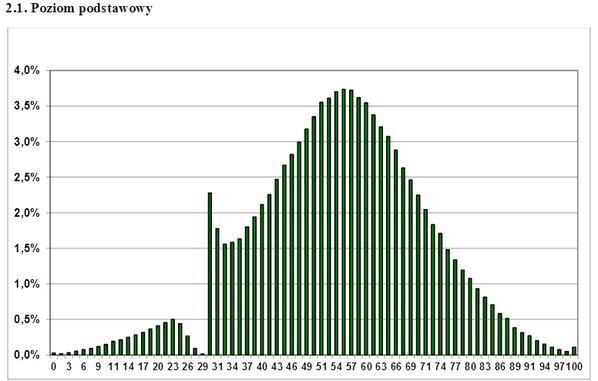
\includegraphics[scale=0.65]{EGE_poland.jpg}
	\end{center}
\end{figure}


\end{document} 
